\graphicspath{{RL/fig}}
\chapter{Dynamic Programming and Reinforcement Learning}
\label{chap:RL}

\section{Introduction}


\section{Dynamic Programming}
\subsection{Introduction}
Dynamic programming is a method to solve problems by using a divide and conquer approach. That is to say a problem is broken into smaller sub-problems and then solved.
There are two properties that must be met for a problem to be solvable via Dynamic Programming: Optimal substructure and Overlapping sub-problems. \cite{David_Silver}
\begin{itemize}
	\item Optimal substructure requires that the solution be able to be decomposed into sub-problems.
	\item Overlapping sub-problems requires that the sub-problems occur many times over, meaning that the solution can be cached and reused.
\end{itemize}

Markov decision processes satisfies both of these conditions. The Bellman equation provides a recursive decomposition which fulfills the Optimal substructure property. While the value function caches and reuses solutions satisfying the Overlapping sub-problems condition. \cite{David_Silver}\\

\subsection{Iterative Policy Evaluation}
In order to evaluate the value that a certain policy has, we use a method called \textit{Iterative Policy Evaluation}. Figure \ref{fig:iterative_policy_evaluation} shows the mathematics which describes Iterative Policy Evaluation in both summation and vector form. What the diagram  at the top of Figure \ref{fig:iterative_policy_evaluation} represents is the value function being calculated for an action 'a' to an intermediary state represented by the black dot. The environments reaction is then also accounted for from the intermediary state to state s' resulting in reward r. The environments information is contained in the transition probability matrix $P^\pi$.

We then use state s' as the new start state s and repeat the same calculation.
The value function is updated continuously until the difference between $v^{k}$ and $v^{k+1}$ is determined negligible.

\begin{figure}
	\centering
	\begin{subfigure}{.49\textwidth}
		\centering
		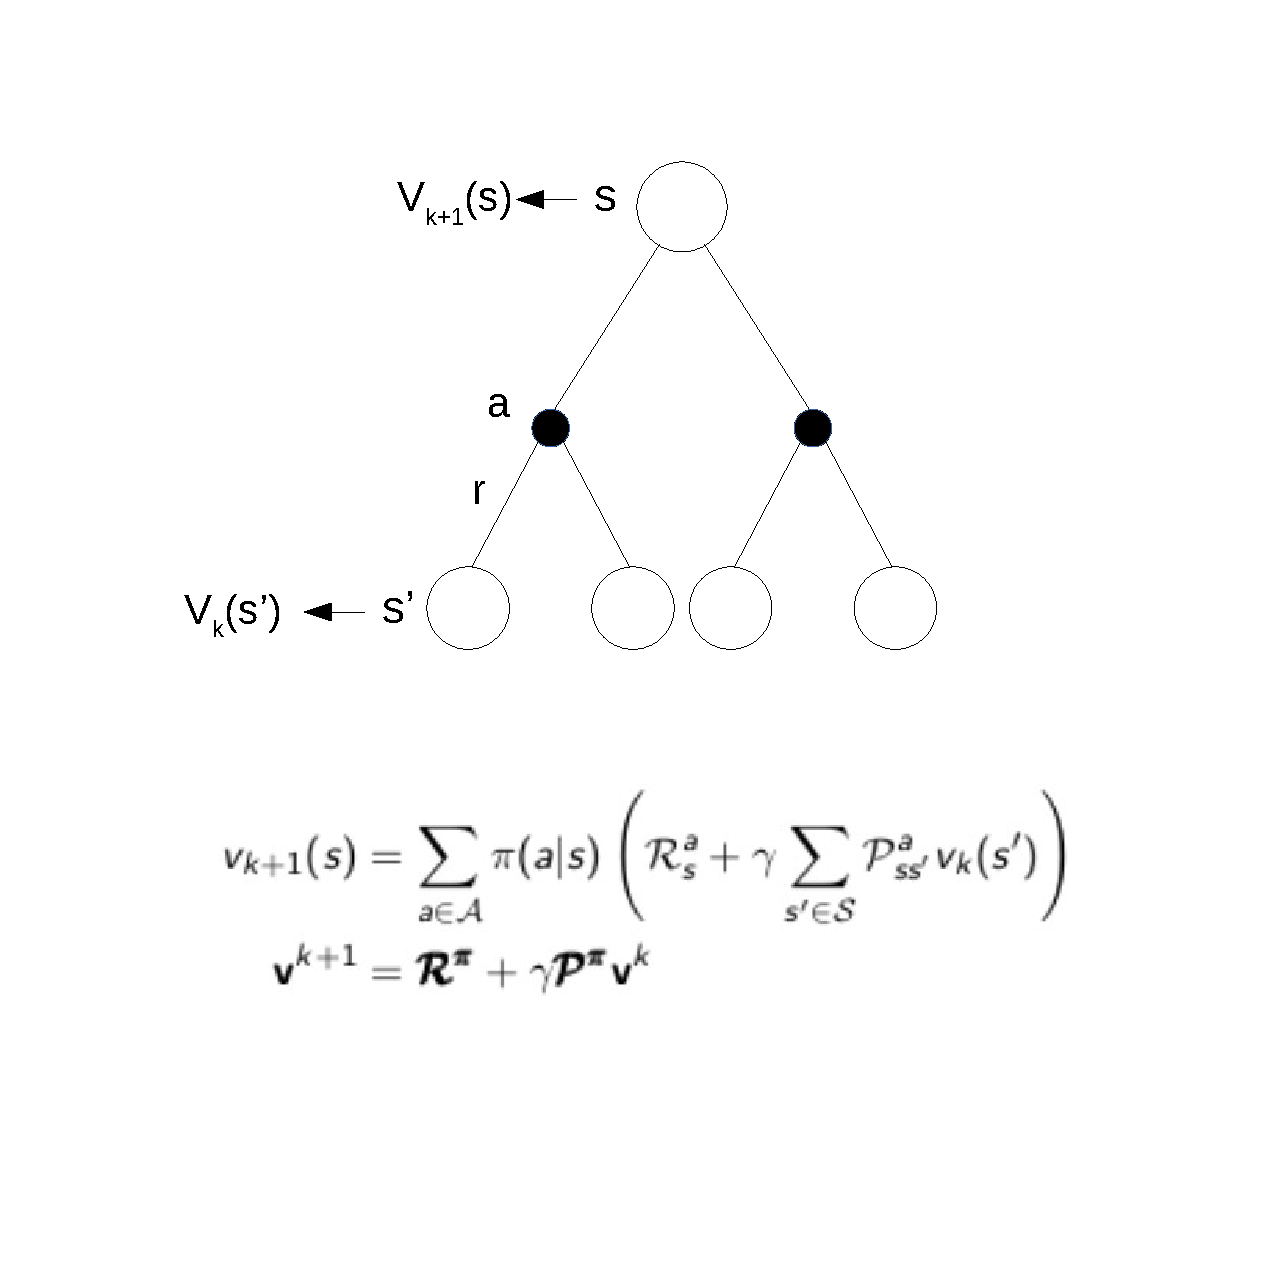
\includegraphics[width=1\linewidth]{MDP_and_DP/fig/Iterative_Policy_Evaluation.png}
		\caption{Iterative policy Evaluation\cite{David_Silver}}
		\label{fig:iterative_policy_evaluation}
	\end{subfigure}
	\begin{subfigure}{.49\textwidth}
		\centering
		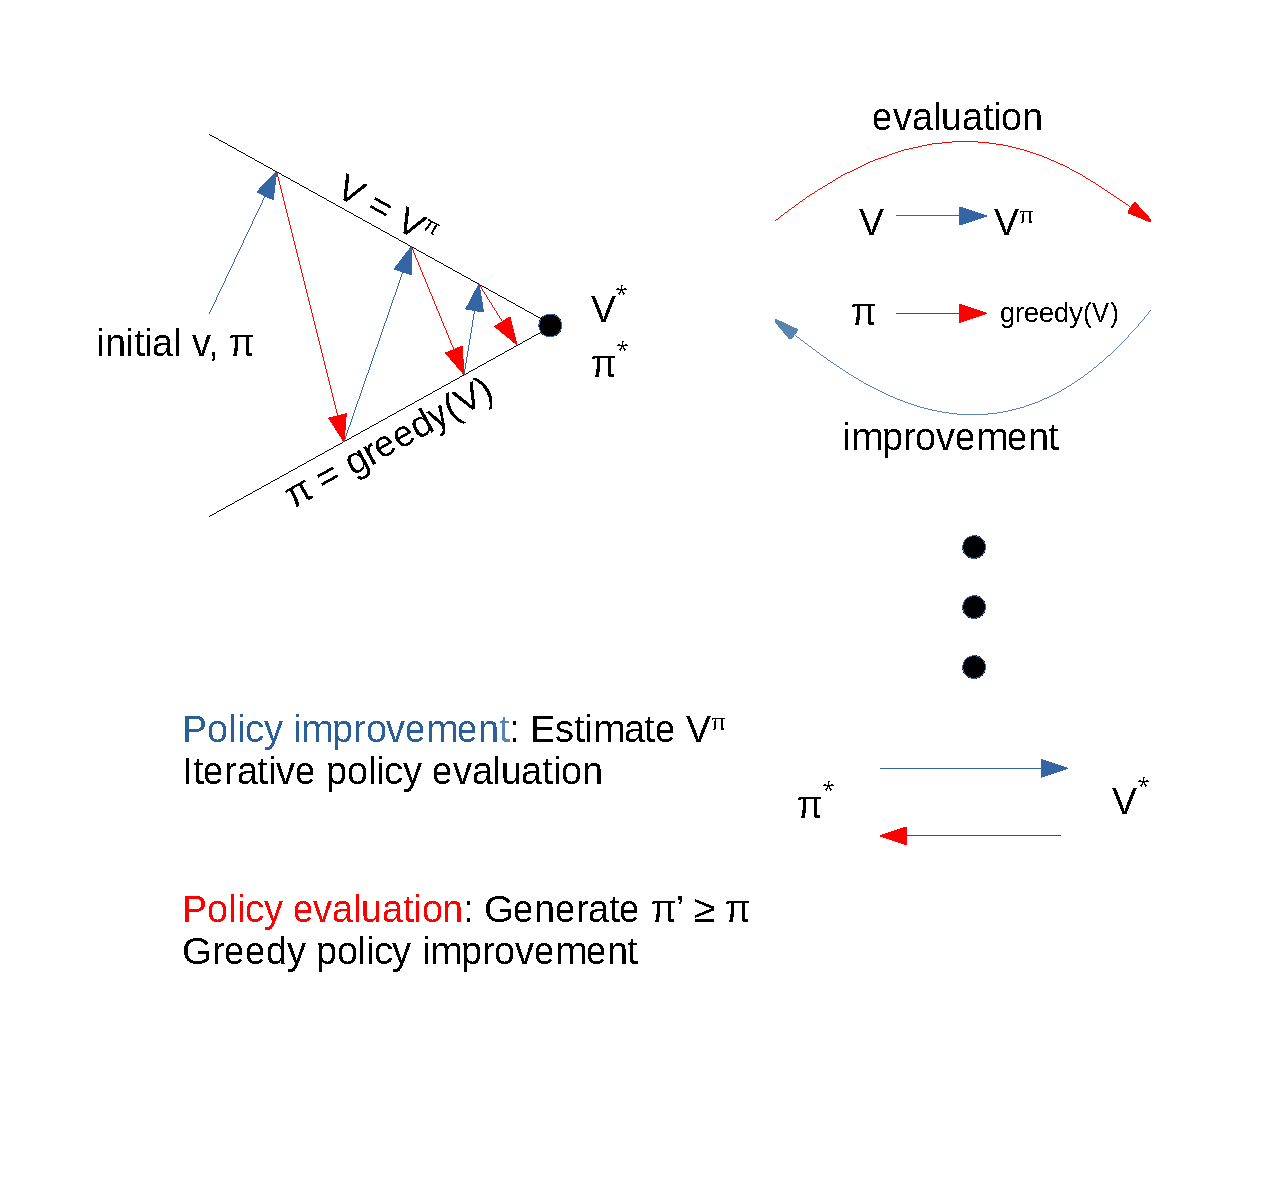
\includegraphics[width=1\linewidth]{MDP_and_DP/fig/Policy_iteration.png}
		\caption{Greedy Policy iteration visualisation\cite{David_Silver}}
		\label{fig:greedy_policy_iteration}
	\end{subfigure}
	\caption{Policy Iteration \cite{David_Silver}}
	\label{fig:policy_iteration}
\end{figure}
\section{Reinforcement Learning}
\subsection{Introduction}
There are two separate uses for Dynamic Programming in Reinforcement Learning. These are prediction and control which both have $(S,A,P,R,\gamma)$ as input.
\begin{itemize}
	\item The prediction method uses $(S,A,P,R,\gamma)$ and a policy $\pi$ as input, while it outputs a value function $v_\pi$.
	\item The control method only takes $(S,A,P,R,\gamma)$ as input and outputs the optimal value function $v_*$ and optimal policy $\pi_{*}$.
\end{itemize}
{\color{red} Maybe insert a flow diagram illustrating difference and similarity between prediction and control }

These two methods of Dynamic programming are implemented via what is known as value iteration and policy iteration respectively.

\subsection{Policy Iteration}

Figure \ref{fig:greedy_policy_iteration} shows how Greedy Policy Iteration works. A greedy policy is one which when followed, results in the maximum value function $v_\pi$. It is known that policy iteration converges which can also be seen in the diagram in Figure \ref{fig:greedy_policy_iteration} on the top left.\cite{sutton_barto}

As is stated in Figure \ref{fig:greedy_policy_iteration} policy iteration works by continuously iterating between two steps, namely policy evaluation and policy improvement.


For a given policy $\pi$ we improve the policy using the following two steps:\\\\
\textbf{Step one} is \textit{Evaluating} the policy $\pi$ using equation \ref{bellmanv2}: \[v_{\pi}(s) = E_{\pi}[R_{t+1} + \gamma v_{\pi}(S_{t+1})|S_t = s]\]
\textbf{Step two} is \textit{Improving} the policy by acting greedy with respect to $v_\pi$ to obtain a new policy $\pi^{'}$:
\[\pi^{'} = greedy(v_{\pi})\]

What this means is that we obtain a value function by using iterative policy evaluation where after we update the policy. In this way we will always converge to the optimal policy $\pi_{*}$ and value function $v_{*}$ described by equation \ref{eq:pi_*} and \ref{bellmanv*} respectively.
\subsection{Value Iteration}
\begin{figure}[!htb]
	\centering
	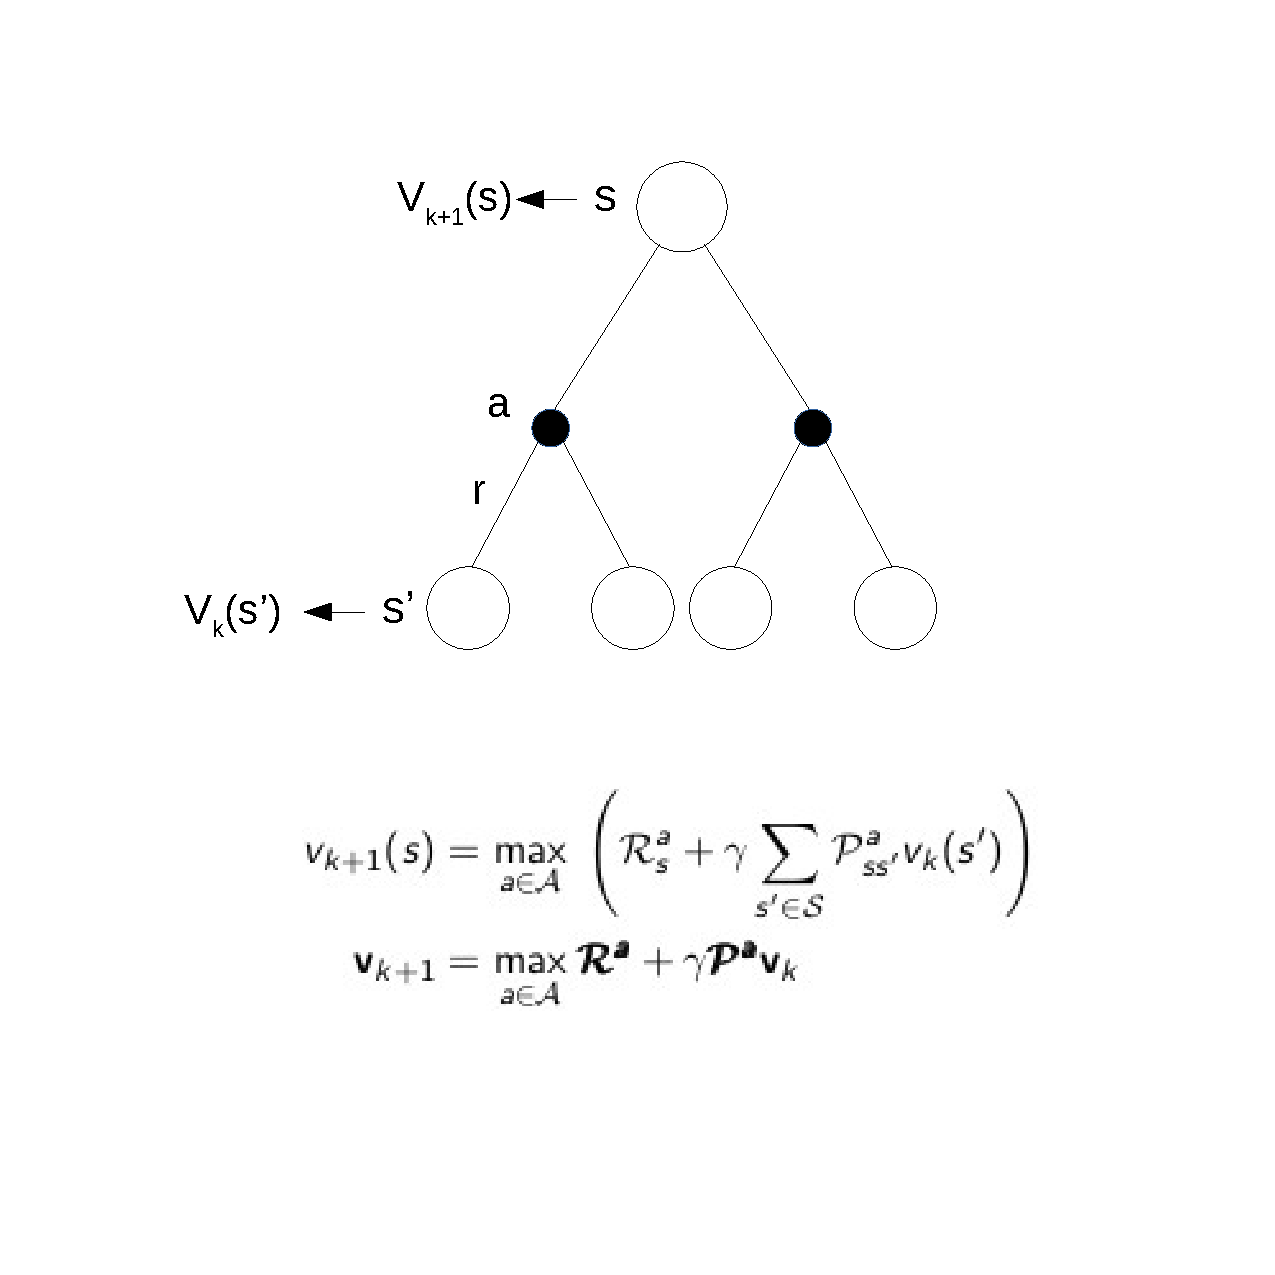
\includegraphics[width=0.75\linewidth]{MDP_and_DP/fig/value_iteration.png}
	\caption{Value Iteration\cite{David_Silver}}
	\label{fig:value_iteration}
\end{figure}
Figure \ref{fig:value_iteration} shows the mathematics that describes \textit{Value Iteration}. It is very similar to iterative policy evaluation in Figure \ref{fig:iterative_policy_evaluation}. Iterative Policy Evaluation calculates the value function for a policy $\pi$ which is an entire set of actions given states.

While Value Iteration calculates the maximum value function for a single action only. In this sense Value Iteration is a special case of Iterative Policy Evaluation.

{\color{red} Can later place in appendix proof of policy iteration always converging. slide 19 (16/42) of David Silvers slides on Dynamic Programming}